\begin{figure}[!ht]
    \centering
    \includegraphics[scale=0.3]{images/legend}
    
    \subfloat[Tempo de execução]{
        \label{Vacation}
        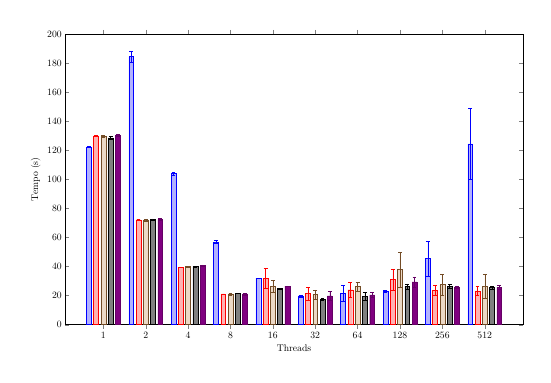
\begin{tikzpicture}[scale=0.35, baseline]
        \begin{axis}[
            width=1.5 \linewidth,
            height=1 \linewidth,
            %media de tempo intruder
            ybar=2.5pt,
            %enlargelimits=0.10,
            % legend style={at={(0.5,-0.15)}, anchor=north, legend columns=-1},
            ylabel=Tempo (s),
            xlabel=Threads,
            symbolic x coords={1, 2, 4, 8, 16, 32, 64, 128, 256, 512},
            xtick=data,
            ymin=0,
            ymax=200,
            bar width=5pt,
            % nodes near coords,
            nodes near coords align={vertical},
        ]
        \addplot+[error bars,y dir=both, y explicit] coordinates {
            (1,122.19)+-(1,0.35) (2,184.47)+-(2,3.93) (4,103.92)+-(4,1.04) (8,56.80)+-(8,1.07) (16,31.99)+-(16,0.24) (32,19.69)+-(32,0.52) (64,21.68)+-(64,5.72) (128,23.22)+-(128,0.57) (256,45.58)+-(256,11.99) (512,124.45)+-(512,24.20) 
        };
        \addplot+[error bars,y dir=both, y explicit] coordinates {
            (1,129.87)+-(1,0.52) (2,72.20)+-(2,0.44) (4,39.59)+-(4,0.19) (8,21.14)+-(8,0.09) (16,31.78)+-(16,6.87) (32,21.39)+-(32,4.41) (64,24.02)+-(64,4.93) (128,31.01)+-(128,7.24) (256,23.53)+-(256,3.50) (512,23.21)+-(512,3.03)
        };
        \addplot+[error bars,y dir=both, y explicit] coordinates {
            (1,129.58)+-(1,0.88) (2,71.87)+-(2,0.48) (4,39.90)+-(4,0.39) (8,21.15)+-(8,0.64) (16,26.35)+-(16,4.18) (32,20.69)+-(32,3.15) (64,26.17)+-(64,3.04) (128,38.12)+-(128,12.03) (256,27.50)+-(256,7.32) (512,26.48)+-(512,8.21)
        };
        \addplot+[error bars,y dir=both, y explicit] coordinates {
            (1,128.56)+-(1,0.95) (2,72.45)+-(2,0.41) (4,40.00)+-(4,0.22) (8,21.55)+-(8,0.22) (16,24.76)+-(16,0.20) (32,17.51)+-(32,0.39) (64,19.62)+-(64,2.71) (128,26.34)+-(128,1.81) (256,26.30)+-(256,1.52) (512,25.59)+-(512,1.05) 
        };
        \addplot+[error bars,y dir=both, y explicit] coordinates {
            (1,130.29)+-(1,0.63) (2,72.49)+-(2,0.59) (4,40.83)+-(4,0.31) (8,21.11)+-(8,0.63) (16,26.56)+-(16,0.15) (32,19.76)+-(32,3.23) (64,20.45)+-(64,1.74) (128,29.49)+-(128,3.46) (256,25.76)+-(256,0.95) (512,25.70)+-(512,1.49)
        };
        % \legend {Tiny, Latency-Sequential, Latency-Chunks, Threshold-Sequential, Threshold-Chunks}
        \end{axis}
        \end{tikzpicture}
    }
    \subfloat[Aborts]{
        \label{abortVacation}
        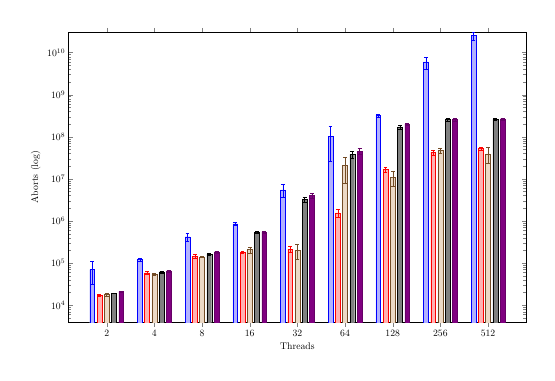
\begin{tikzpicture}[scale=0.35, baseline]
        \begin{axis}[
            ymode=log,
            width=1.5 \linewidth,
            height=1 \linewidth,
            %media de tempo intruder
            ybar=2.5pt,
            %enlargelimits=0.10,
            % legend style={at={(0.5,-0.15)}, anchor=north, legend columns=-1},
            ylabel=Aborts (log),
            xlabel=Threads,
            symbolic x coords={1, 2, 4, 8, 16, 32, 64, 128, 256, 512},
            xtick=data,
            ymin=0,
            ymax=31000000000,
            bar width=5pt,
            % nodes near coords,
            nodes near coords align={vertical},
        ]
        \addplot+[error bars,y dir=both, y explicit] coordinates {
            (1,0.0)+-(1,0.0) (2,69940.4)+-(2,38859.442881235445) (4,123224.4)+-(4,10230.047558051723) (8,421702.0)+-(8,83144.47432752221) (16,858817.0)+-(16,70319.27963794851) (32,5482927.6)+-(32,1822574.306164838) (64,102125071.2)+-(64,75531726.60526115) (128,324906951.0)+-(128,25833176.356745664) (256,5976414236.0)+-(256,1965369780.1742249) (512,25331573456.2)+-(512,5125278647.27645) 
        };
        \addplot+[error bars,y dir=both, y explicit] coordinates {
            (1,0.0)+-(1,0.0) (2,17295.8)+-(2,884.117051074121) (4,58832.4)+-(4,5182.0950049183775) (8,145328.0)+-(8,14502.15570182585) (16,179942.6)+-(16,9939.803108713975) (32,213282.4)+-(32,33756.78063204487) (64,1563534.8)+-(64,303501.08637854987) (128,16550448.4)+-(128,2123035.5644618487) (256,42956098.2)+-(256,6012180.935710481) (512,52269879.0)+-(512,4755551.76397057)
        };
        \addplot+[error bars,y dir=both, y explicit] coordinates {
             (1,0.0)+-(1,0.0) (2,17786.7)+-(2,1249.259304548099) (4,54750.2)+-(4,2738.370420523856) (8,141273.5)+-(8,6123.819286197136) (16,209526.5)+-(16,34736.26421551402) (32,201599.3)+-(32,81127.76465680539) (64,20569626.4)+-(64,12875680.754533986) (128,10897558.0)+-(128,4040389.7657925775) (256,46668204.777777776)+-(256,5450523.901092766) (512,39389491.0)+-(512,16022591.920577014) 
        };
        \addplot+[error bars,y dir=both, y explicit] coordinates {
            (1,0.0)+-(1,0.0) (2,19074.2)+-(2,369.0059078117856) (4,61648.4)+-(4,2902.3763091646124) (8,161693.8)+-(8,9525.331540686655) (16,536547.4)+-(16,18869.180433712536) (32,3237316.8)+-(32,385306.9331768636) (64,38103581.6)+-(64,7477543.014654762) (128,171013189.4)+-(128,21848968.54501459) (256,256035773.6)+-(256,17482704.25370147) (512,263634097.2)+-(512,12981014.911830684)
        };
        \addplot+[error bars,y dir=both, y explicit] coordinates {
            (1,0.0)+-(1,0.0) (2,21093.1)+-(2,312.0) (4,64726.72)+-(4,3041.77) (8,183647.1)+-(8,8673.62) (16,544787.54)+-(16,23782.8) (32,3980021.4)+-(32,552484.0028907986) (64,45836278.2)+-(64,6287845.41) (128,199521897.4)+-(128,10431600.060439752) (256,254781534.6)+-(256,19017136.502195936) (512,266950650.75)+-(512,14874593.300939599)
        };
        % \legend {Tiny, Latency-Sequential, Latency-Chunks, Threshold-Sequential, Threshold-Chunks}
        \end{axis}
        \end{tikzpicture}
    }
\end{figure}
